\documentclass[10pt,twocolumn,a4paper]{article}

\usepackage{cvpr}
\usepackage{times}
\usepackage{epsfig}
\usepackage{graphicx}
\usepackage{amsmath}
\usepackage{amssymb}
\usepackage{algpseudocode}

% Include other packages here, before hyperref.

% If you comment hyperref and then uncomment it, you should delete
% egpaper.aux before re-running latex.  (Or just hit 'q' on the first latex
% run, let it finish, and you should be clear).
\usepackage[breaklinks=true,bookmarks=false]{hyperref}

\cvprfinalcopy % *** Uncomment this line for the final submission

\def\cvprPaperID{****} % *** Enter the CVPR Paper ID here
\def\httilde{\mbox{\tt\raisebox{-.5ex}{\symbol{126}}}}

% Pages are numbered in submission mode, and unnumbered in camera-ready
%\ifcvprfinal\pagestyle{empty}\fi
\setcounter{page}{1}
\begin{document}

%%%%%%%%% TITLE
\title{Perceptron for Predicting Diabetes}

\author{Christopher Hamilton\\
The University of Adelaide\\
{\tt\small christopher.hamilton@student.adelaide.edu.au}
% For a paper whose authors are all at the same institution,
% omit the following lines up until the closing ``}''.
% Additional authors and addresses can be added with ``\and'',
% just like the second author.
% To save space, use either the email address or home page, not both
}

\maketitle
%\thispagestyle{empty}

%%%%%%%%% ABSTRACT
\begin{abstract}
   The is to be in fully-justified italicized text, at the top
   of the left-hand column, below the author and affiliation
   information. Use the word ``Abstract'' as the title, in 12-point
   Times, boldface type, centered relative to the column, initially
   capitalized. The abstract is to be in 10-point, single-spaced type.
   Leave two blank lines after the Abstract, then begin the main text.
   Look at previous CVPR abstracts to get a feel for style and length.
\end{abstract}

%%%%%%%%% BODY TEXT
\section{Introduction}

The prediction of diabetes in individuals without the need for specialised
testing may be beneficial for the early diagnoses of the disease as well
as increasing the number of people who get tested. Given a set of data
relating to a person's health, we may be able to accurately identify
whether or not that individual has diabetes, without the need for a
specific blood test. The set of variables available in the dataset includes
the number of pregnancies, glucose concentration in an oral glucose
concentration test, blood pressure, skin thickness, insulin level, BMI,
diabetes pedigree function and age. These independent variables act as
predictor variables for the single dependent, outcome variable in the
dataset, whether or not the individual has diabetes. As the prediction
is either the individual having diabetes or not, the problem to be solved
is a binary classification problem.

A single perceptron is able to classify data into two classes through linear
separation of the data. The classification is done through the use of a
weighted sum that has a threshold applied and depending on if the sum is
over or under the threshold, the data is classified into either of the classes.

\section{Method}

The perceptron is an adaptive system that is able to recognise patterns in data as well as model the functions of the brain. It was first implemented in 1957 by Frank Rosenblatt at Cornell Aeronautical Laboratory as a way to classify inputs without the need for human action, similar to the human brain. Through research into the physical nervous system and the human brain, discoveries have been made into neuron pathways, and how neurons interact with one another. In humans, it has been discovered that the initial network of connections between neurons is mostly random and as neural activity occurs during development, the reactions of cells to a stimulus changes. Another key result that was found is that when a many stimuli are applied, connections are often formed between the same sets of neurons for similar stimuli and are formed between different sets of neurons for stimuli that are unalike. 

These discoveries have been applied in the development of the perceptron for the binary classification of data. The result of the similar stimuli causing activation for similar neurons has been taken and from this, the perceptron has been designed to classify data to the same class that similar training data was labelled as. A perceptron takes in an input of multiple variables, and based on a set of weights that it has been trained for, generates a weighted sum of these variables. For a perceptron, this weighted sum is used to classify the output into either of the two possible classes, if the sum is greater than or equal to 0, the will be given the positive class (+1) and if it is less than 0, it will be given the negative class (-1).

In order for the perceptron to be able to accurately classify data, it must have weights trained based on a set of inputs which are labelled with correct classes already. The perceptron training algorithm involves setting all weights incorrectly at first, and then iteratively updating the weights based on the product of the training class and the training input data. This algorithm can be written mathematically as:

Assume:
\[ g(\vec{x}; \vec{w}) = sign(\vec{x} \cdot \vec{w}) \]
Where $ \vec{x},\vec{w} \in \mathbb{R}^d $, and $y \in \{-1, 1\} $

For a set of training data: $ \{(\vec{x_i}, y_i)\}_{i=1}^n $,

a step size: $\eta$,

and a number of iterations $T$

The perceptron training algorithm is as follows:
\begin{algorithmic}
\State $\vec{w} \gets \vec{0}$
\For{$t=1$ to $T$}

    $\vec{w_{t+1}} = \vec{w_t} + \eta \sum_{i=1}^n(y_i \vec{x_i} 1_{\{ y_i (\vec{x_i} \cdot \vec{w_t}  ) \leq 0 \}})$
\EndFor
\end{algorithmic}

We denote the trained weights of the perceptron as $w^*$ and this is the same as $w_T$, the weights as updated at the end of the final epoch.

Prediction using this trained perceptron is then done by taking the dot product between the input vector and the weights, to produce a predicted class label, $y^* \in \{-1, 1\}$.

\[ g(\vec{x}; \vec{w^*}) = y^* = sign(\vec{x} \cdot \vec{w^*} ) \]

Since a weighted sum is used as the input to the perceptron, computers are able to very quickly perform the dot products and summations required for the training of a perceptron, as well as the classification of data. This makes the method very useful to quickly classify linearly separable data into one of two classes, given that the weights have been appropriately set to separate the data for the problem to be solved.

The perceptron while able to converge to a prediction for linearly separable data, has some limitations. The first limitation of the perceptron algorithm is that it is only able to converge if the data is linearly separable. This limits the use cases that the perceptron has, a simple example of this is shown in Figure \ref{fig:non-linearly-separable}.

\begin{figure}
    \centering
    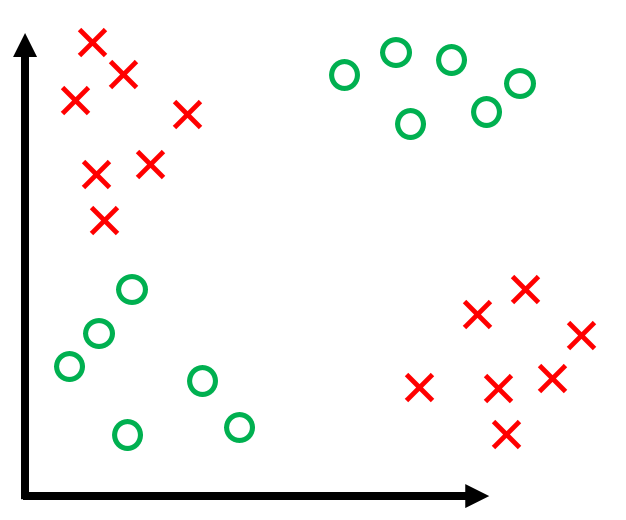
\includegraphics[width=1\linewidth]{non-linearly-separable.png}
    \caption{Example of non-linearly separable data}
    \label{fig:non-linearly-separable}
\end{figure}

The data contains two classes, but these cannot be linearly separated, any line drawn to separate the points in this two dimensional space will result in some of the data points being classified incorrectly.

Another limitation of the perceptron is that it is only able to perform binary classification, and this results in only two options for the predicted class. This works well in data sets where the outcome variable is some sort of indicator variable, however for other use cases, such as data that needs to be classified into three classes, it will not work.


%-------------------------------------------------------------------------
\subsection{Margins and page numbering}

All printed material, including text, illustrations, and charts, must be kept
within a print area 6-7/8 inches (17.5 cm) wide by 8-7/8 inches (22.54 cm)
high.
Page numbers should be in footer with page numbers, centered and .75
inches from the bottom of the page and make it start at the correct page
number rather than the 4321 in the example.  To do this fine the line (around
line 23)
\begin{verbatim}
%\ifcvprfinal\pagestyle{empty}\fi
\setcounter{page}{4321}
\end{verbatim}
where the number 4321 is your assigned starting page.

Make sure the first page is numbered by commenting out the first page being
empty on line 46
\begin{verbatim}
%\thispagestyle{empty}
\end{verbatim}


%-------------------------------------------------------------------------
\subsection{Type-style and fonts}

Wherever Times is specified, Times Roman may also be used. If neither is
available on your word processor, please use the font closest in
appearance to Times to which you have access.

MAIN TITLE. Center the title 1-3/8 inches (3.49 cm) from the top edge of
the first page. The title should be in Times 14-point, boldface type.
Capitalize the first letter of nouns, pronouns, verbs, adjectives, and
adverbs; do not capitalize articles, coordinate conjunctions, or
prepositions (unless the title begins with such a word). Leave two blank
lines after the title.

AUTHOR NAME(s) and AFFILIATION(s) are to be centered beneath the title
and printed in Times 12-point, non-boldface type. This information is to
be followed by two blank lines.

The ABSTRACT and MAIN TEXT are to be in a two-column format.

MAIN TEXT. Type main text in 10-point Times, single-spaced. Do NOT use
double-spacing. All paragraphs should be indented 1 pica (approx. 1/6
inch or 0.422 cm). Make sure your text is fully justified---that is,
flush left and flush right. Please do not place any additional blank
lines between paragraphs.

Figure and table captions should be 9-point Roman type as in
Figures~\ref{fig:onecol} and~\ref{fig:short}.  Short captions should be centred.

\noindent Callouts should be 9-point Helvetica, non-boldface type.
Initially capitalize only the first word of section titles and first-,
second-, and third-order headings.

FIRST-ORDER HEADINGS. (For example, {\large \bf 1. Introduction})
should be Times 12-point boldface, initially capitalized, flush left,
with one blank line before, and one blank line after.

SECOND-ORDER HEADINGS. (For example, { \bf 1.1. Database elements})
should be Times 11-point boldface, initially capitalized, flush left,
with one blank line before, and one after. If you require a third-order
heading (we discourage it), use 10-point Times, boldface, initially
capitalized, flush left, preceded by one blank line, followed by a period
and your text on the same line.

%-------------------------------------------------------------------------
\subsection{Footnotes}

Please use footnotes\footnote {This is what a footnote looks like.  It
often distracts the reader from the main flow of the argument.} sparingly.
Indeed, try to avoid footnotes altogether and include necessary peripheral
observations in
the text (within parentheses, if you prefer, as in this sentence).  If you
wish to use a footnote, place it at the bottom of the column on the page on
which it is referenced. Use Times 8-point type, single-spaced.


%-------------------------------------------------------------------------
\subsection{References}

List and number all bibliographical references in 9-point Times,
single-spaced, at the end of your paper. When referenced in the text,
enclose the citation number in square brackets, for
example~\cite{Authors14}.  Where appropriate, include the name(s) of
editors of referenced books.

\begin{table}
\begin{center}
\begin{tabular}{|l|c|}
\hline
Method & Frobnability \\
\hline\hline
Theirs & Frumpy \\
Yours & Frobbly \\
Ours & Makes one's heart Frob\\
\hline
\end{tabular}
\end{center}
\caption{Results.   Ours is better.}
\end{table}

%-------------------------------------------------------------------------
\subsection{Illustrations, graphs, and photographs}

All graphics should be centered.  Please ensure that any point you wish to
make is resolvable in a printed copy of the paper.  Resize fonts in figures
to match the font in the body text, and choose line widths which render
effectively in print.  Many readers (and reviewers), even of an electronic
copy, will choose to print your paper in order to read it.  You cannot
insist that they do otherwise, and therefore must not assume that they can
zoom in to see tiny details on a graphic.

When placing figures in \LaTeX, it's almost always best to use
\verb+\includegraphics+, and to specify the  figure width as a multiple of
the line width as in the example below
{\small\begin{verbatim}
   \usepackage[dvips]{graphicx} ...
   \includegraphics[width=0.8\linewidth]
                   {myfile.eps}
\end{verbatim}
}


%-------------------------------------------------------------------------
\subsection{Color}

Please refer to the author guidelines on the CVPR 2020 web page for a discussion
of the use of color in your document.

%------------------------------------------------------------------------
\section{Final copy}

You must include your signed IEEE copyright release form when you submit
your finished paper. We MUST have this form before your paper can be
published in the proceedings.

Please direct any questions to the production editor in charge of these 
proceedings at the IEEE Computer Society Press: 
\url{https://www.computer.org/about/contact}. 


{\small
\bibliographystyle{ieee_fullname}
\bibliography{egbib}
}

\end{document}
